\hypertarget{introduction}{%
\chapter{Introduction}\label{introduction}}
This document is written for the participants of the students laboratory
``Developing Embedded Application Specific Processors'', that is offered
at the Chair for Embedded Systems \cite{CES} at Karlsruhe Institute of
Technology (KIT). This document assumes a tool- and environment-setup
specific to this laboratory. Many parts are written keeping our
development environment in mind and cannot be applied to other setups
without change, but users of such setups can get an impression about the
tool chains for specific tasks.

\hypertarget{application-specific-instruction-set-processors}{%
\section{Application Specific Instruction Set
Processors}\label{application-specific-instruction-set-processors}}
Application Specific Instruction-set Processors (ASIPs) are a good
trade-off between Application Specific Integrated Circuits (ASICs) and
General Purpose Processors (GPPs). ASICs show the best performance in
energy and speed, but on the other hand, they have the highest
development costs and therefore are only reasonable for high volume
products. Unlike ASICs, where everything is executed in hardware, GPPs
execute everything in software. This makes them extremely flexible, but
on the other hand, they show a bad performance in energy and speed
terms, especially compared to ASICs.

ASIPs are processors with an application specific instruction set. So,
in contrast to the GPPs they are optimized for a specific application or
for a group of applications. For this group of applications they achieve
better energy and speed results than GPPs, as they have hardware support
for these applications. However, contrary to ASICs they are still very
flexible and can execute any kind of application, although they do not
have the energy and speed benefits for other applications. The
customization of ASIPs typically addresses three architectural levels
that vary depending on the platform vendor \cite{Henkel03}:
\begin{itemize}
\item
  \emph{Instruction extension}: The designer can define customized
  instructions by specifying their functionality. The extensible
  processor platform will then generate the extended instructions that
  then coexist with the base instruction set.
\item
  \emph{Inclusion/exclusion of predefined blocks}: The designers can
  choose to include or exclude predefined blocks as part of the
  extensible processor platform. Block examples include special function
  registers, built-in self-test, multiply-and-accumulate operation
  blocks, and caches.
\item
  \emph{Parameterization}: The designer can fix extensible processor
  parameters such as instruction and data cache sizes, the number of
  registers, and so on.
\end{itemize}
\begin{figure}[!htb]
	\centering
	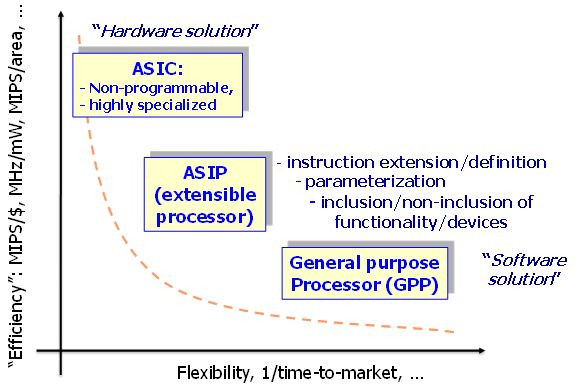
\includegraphics[width=0.9\textwidth]{src/images/1-1.png}
	\caption{ GPPs, ASIPs and ASICs \cite{Henkel06}}
	\label{fig:fig11}
\end{figure}
ASIPs represent a good trade-off between Application Specific Integrated
Circuits (ASICs) and General Purpose Processors (GPPs), as shown in Figure
\ref{fig:fig11}. ASICs have the highest efficiency
due to the fact, that they are often manually optimized for a specific
task and therefore only the necessary elements are included. This has a
high impact to the power consumption and the execution speed, but it
causes a high time-to-market and high development costs. Nevertheless,
these development costs can amortize when selling a huge amount of
units, due to the lower costs per unit. The GPPs are less efficient due
to the fact, that they are usable for many different kinds of
applications and therefore often contain blocks that are not needed for
a certain task. Whenever an application domain changes frequently due to
e.g. changing standards, then the GPPs are capable to adapt to these
changes, whereas the ASIC would need to be redesigned.
\hypertarget{asip-design-flow}{%
\section{ASIP Design Flow}\label{asip-design-flow}}
Designing an ASIP typically starts with analyzing and profiling the
targeted application or application domain, as shown in Figure
\ref{fig:fig12}. After this analysis, an ASIP is
defined by e.g. specifying its instructions set, embedding blocks that
are required to implement the instructions, and further configuring the
architecture. Traditionally, the step of defining the ASIP is done
manually. However, recent research activities have focused on automating
this process within the range of a manually defined search space.

After the ASIP is defined, a synthesizable hardware description (for
implementing the ASIP) and a tool chain (e.g. compiler, simulator, etc.)
are created automatically. Using these tools and the hardware
description, the ASIP is simulated and benchmarked. This might lead to a
refinement of the ASIP to further optimize it or to keep the
constraints, e.g. the area- or power budget. After the ASIP fulfills the
requirements, a prototype (e.g. FPGA-based) is created and finally, the
ASIP is taped out.
\begin{figure}[!htb]
	\centering
	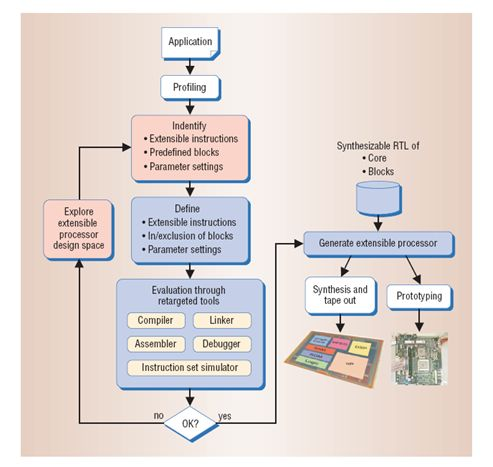
\includegraphics[width=0.9\textwidth]{src/images/1-2.png}
	\caption{Typical ASIP Design Flow \cite{Henkel03}}
	\label{fig:fig12}
\end{figure}
\hypertarget{custom-instruction-identification}{%
\section{Custom Instruction
Identification}\label{custom-instruction-identification}}
Custom Instructions often combine often-executed functionality in one
dedicated assembler instruction. That allows executing this
functionality faster and/or more efficient, etc. Generally, there are
two ways to improve the performance by using Custom Instructions:
\begin{itemize}
\item
  Parallelism: Execute multiple operations that are (data-wise)
  independent from each other in parallel (i.e. at the same time)
\item
  Chaining: Execute multiple operations that are (data-wise) dependent
  from each other sequentially (i.e. after each other) but within the
  same cycle. This might affect the frequency of the ASIP (to assure
  that all operations complete in the same cycle).
\end{itemize}
Both, parallelism and chaining can be applied together in the same
Custom Instruction. Furthermore, sometimes it may also be beneficial to
consider a very different implementation (compared to the given software
implementation of the application) that results in the same
functionality. For instance, to exchange two Bytes within the same Word,
a software implementation has to use \emph{and}, \emph{shift}, and
\emph{or} operations. However, in hardware this corresponds to a simple
re-wiring without any computation and thus can be implemented very
efficient.

There are some constraints for defining Custom Instructions. A Custom
Instruction is typically an unbreakable operation, i.e. it is executed
either completely or not at all. Therefore, the same property has to
hold for the part of the application that is considered to become a
Custom Instruction. An application consist of a certain control flow and
a data flow. The control flow is realized by jumps, loops, etc. The data
flow instead corresponds to the input- and output dependencies of the
operations. An application can be represented as a so-called Base-Block
graph. A Base Block thereby represents a set of operations that are
always executed together (more formally: a sequence of operations that
does not contain a \emph{jump} except at its end and where no
\emph{jump} may enter the sequence except at its beginning). A Base
Block fulfills the above-mentioned requirements of an unbreakable
operation and therefore is a good candidate for a Custom Instruction.
However, sometimes it is possible to embed control flow within a Custom
Instruction. For instance in the case of a MAX operation (i.e.
determining the maximum of two values and assigning it to a result
variable), both control-flow parts (the \emph{then} and the \emph{else}
part) can be embedded inside the Custom Instruction.

There are further constraints that are important when identifying Custom
Instruction. They will be explained by using the example shown in Figure
\ref{fig:fig13}. Part a) shows a given data flow
within a Base Block (i.e. no further control flow limits the selection
of a Custom Instruction) that is executed very frequently in an
application (and thus is an interesting candidate for a Custom
Instruction). Each node in this graph corresponds to a certain operation
(e.g., addition) and the edges correspond to data dependencies. The
first approach is to try to implement the whole data flow as one rather
larger Custom Instruction. If the critical path of this data flow is too
long (and thus would affect the frequency of the ASIP) the data flow can
be implemented as a so-called multi-cycle operation, i.e. it may require
multiple cycles to execute this instruction (the CPU pipeline is then
typically stalled until the execution completes).

One typical constraint for a Custom Instruction is the amount of
inputs/outputs that are read from/written to the register file. If we
assume that our ASIP provides four read ports and two write ports then
the shown Custom Instruction exceeds these limits. Therefore, we exclude
some nodes of the data flow in part b) of the figure to fulfill the
input/output requirements. Furthermore, there might be so-called
forbidden nodes, i.e. nodes in the data flow that may not be part of a
Custom Instruction. In our example, we have a \emph{load} node, i.e. an
access to the data memory. If we assume that our instruction executes in
the EXE stage of a simple processor pipeline then it might be
complicated to access the resources of the MEM stage to provide access
to the data memory. Therefore, load/store nodes might be forbidden
within a Custom Instruction. In part c) we therefore exclude the
\emph{load} node. However, our Custom Instruction would then no longer
be convex, i.e. we have an edge leaving our Custom Instruction towards a
sub graph (the single \emph{load} node in our example) and another edge
coming from this sub graph and entering our Custom Instruction.
Therefore, our Custom Instruction has to be executed {before} the sub
graph (to provide its input) and {after} the sub graph (to receive its
output) which is obviously not possible at the same time.
\begin{figure}[!htb]
	\centering
	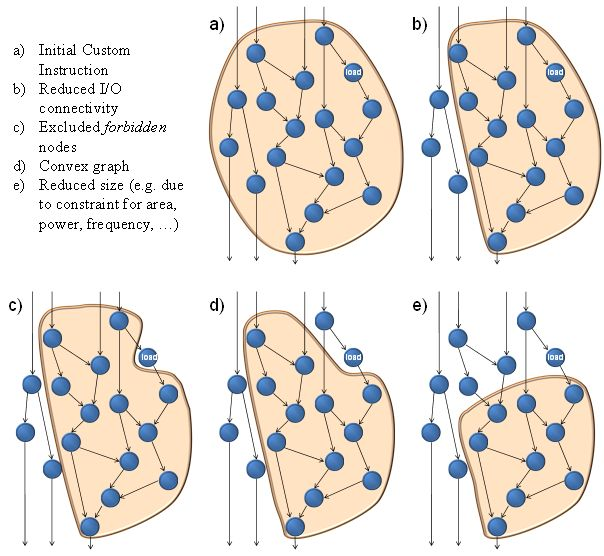
\includegraphics[width=0.9\textwidth]{src/images/1-3.png}
	\caption{Constraints for \emph{valid} Custom Instructions}
	\label{fig:fig13}
\end{figure}
To establish the property of a convex Custom Instruction we exclude
further nodes and reach part d) of Figure \ref{fig:fig13}. This Custom Instruction now is
convex, does not contain \emph{forbidden} nodes, and respects the
maximal input/output ports of the register file. Therefore, it is a
\emph{valid} Custom Instruction. Further constraints (e.g. the maximum
area, power consumption, or latency) might lead to a further reduction
of the data flow graph, as shown in part e).
\hypertarget{goal-of-the-laboratory}{%
\section{Goal of the Laboratory}\label{goal-of-the-laboratory}}
This laboratory will teach the creation of ASIPs from the design, over
the high-level simulation to the final prototype on FPGA hardware.
Benchmarks of speed, needed area and power/energy consumption will be
performed and compared among different created ASIPs. For this purpose
the usage of the different tools have to be practiced and the connection
of these tools to form a tool chain has to be understood. The main goal
is creating new ASIPs for special applications, to benchmark these ASIPs
to find out their benefits and drawbacks and finally to interpret the
benchmark results.
